% !TEX TS-program = pdflatex
% !TEX encoding = UTF-8 Unicode

% This is a simple template for a LaTeX document using the "article" class.
% See "book", "report", "letter" for other types of document.

\documentclass[11pt]{article}

\usepackage[utf8]{inputenc} % set input encoding (not needed with XeLaTeX)

%%% Examples of Article customizations
% These packages are optional, depending whether you want the features they provide.
% See the LaTeX Companion or other references for full information.

%%% PAGE DIMENSIONS
\usepackage{geometry} % to change the page dimensions
\geometry{letterpaper} % or letterpaper (US) or a5paper or....

\usepackage[]{graphicx} % support the \includegraphics command and options

% \usepackage[parfill]{parskip} % Activate to begin paragraphs with an empty line rather than an indent

%%% PACKAGES
\usepackage{booktabs} % for much better looking tables
\usepackage{array} % for better arrays (eg matrices) in maths
\usepackage{paralist} % very flexible & customisable lists (eg. enumerate/itemize, etc.)
\usepackage{verbatim} % adds environment for commenting out blocks of text & for better verbatim
\usepackage{subfig} % make it possible to include more than one captioned figure/table in a single float
% These packages are all incorporated in the memoir class to one degree or another...
\usepackage{mathtools}
\usepackage{listings}
\usepackage{amsmath}
\usepackage{setspace}
\doublespacing
% or:
%\onehalfspacing
%\usepackage[authoryear]{natbib}
\usepackage{hyperref}
\usepackage{float}
\usepackage{epsfig}
\usepackage{import}



%%% HEADERS & FOOTERS
\usepackage{fancyhdr} % This should be set AFTER setting up the page geometry
\pagestyle{fancy} % options: empty , plain , fancy
\renewcommand{\headrulewidth}{0pt} % customise the layout...
\lhead{}\chead{}\rhead{}
\lfoot{}\cfoot{\thepage}\rfoot{}

%%% SECTION TITLE APPEARANCE
\usepackage{sectsty}
\allsectionsfont{\sffamily\mdseries\upshape} % (See the fntguide.pdf for font help)
% (This matches ConTeXt defaults)

%%% ToC (table of contents) APPEARANCE
\usepackage[nottoc,notlof,notlot]{tocbibind} % Put the bibliography in the ToC
\usepackage[titles,subfigure]{tocloft} % Alter the style of the Table of Contents
\renewcommand{\cftsecfont}{\rmfamily\mdseries\upshape}
\renewcommand{\cftsecpagefont}{\rmfamily\mdseries\upshape} % No bold!
\usepackage{datetime}

\newdateformat{mydate}{\monthname[\THEMONTH] \THEYEAR}

%%% END Article customizations

%%% The "real" document content comes below...

%%% END Article customizations

%%% The "real" document content comes below...

\title{THE MILLIMETER-WAVELENGTH SULFUR DIOXIDE ABSORPTION SPECTRA MEASURED UNDER SIMULATED VENUS CONDITIONS }
\author{A Masters Thesis Proposal\\
Presented to\\
The Academic Faculty \\
by \\
Amadeo Bellotti}
\date{\mydate\today} % Activate to display a given date or no date (if empty),
         % otherwise the current date is printed 

\begin{document}
\maketitle

\begin{abstract}
The objective of the proposed research is to develop a mathematical model that accurately estimates the opacity of sulfur dioxide in a carbon dioxide atmosphere under conditions characteristic of the Venus troposphere based on extensive laboratory measurements. High precision measurements of the millimeter-wavelength properties of sulfur dioxide are being conducted under multiple pressure and temperatures. These measurements are being conducted in both W-band and F-band (2-3 and 3-4 millimeter-wavelengths). The results of this research will significantly improve the understanding of the millimeter-wavelength emission spectrum of Venus and possibly determine the source of variations in the Venus millimeter-wavelength emissions. 
\end{abstract}
\newpage
\chapter{Introduction}

%\section{Introduction}
Active and passive microwave remote sensing techniques have been extensively used in the study of our sister planet, Venus. Unlike Earth's atmosphere, the Venus atmosphere is mostly comprised of gaseous carbon dioxide (CO$_2$). CO$_2$ comprises 96.5\% of the atmosphere along with gaseous nitrogen (N$_2$) at about 3.5\%. The Venus atmosphere has multiple trace constituents such as sulfur dioxide (SO$_2$), carbon monoxide (CO), water vapor (H$_2$O), carbonyl sulfide (OCS), and sufuric acid vapor (H$_2$SO$_4$) \cite{Suleiman-thesis}.

Two sulfur-bearing compounds dominate the millimeter-wave emission from Venus: sulfur dioxide (SO$_2$) and gaseous sulfuric acid (H$_2$SO$_4$). At higher pressures H$_2$SO$_4$ thermally dissociates, forming H$_2$O and SO$_3$, both of which exhibit relatively small amounts of microwave absorption at the abundance levels present in the Venus atmosphere. Thus, in the deep atmosphere, only SO$_2$ and CO$_2$ have the potential to affect the observed microwave emission.

Utilizing the millimeter-wavelength system at the Planetary Atmospheres Laboratory at Georgia Institute of Technology, it has been possible to simulate the upper troposphere of Venus and take precision measurements of the millimeter-wavelength properties of sulfur dioxide. Using the measurements, a model that accurately predicts the opacity of sulfur dioxide in the Venus atmosphere has been verified. Applying this opacity model to a newly developed radiative transfer model will make it possible to determine the source of variations in the Venus millimeter-wavelength emission, such as were observed by Sagawa \cite{Sagawa-2008}.

\section{Background and Motivation}

Radio absorptivity data from planetary atmospheres can be used to infer abundances of microwave absorbing constituents. Such data is obtained from entry probe radio signal absorption measurements, spacecraft radio occultation experiments, and earth-based or spacecraft based radio emission observations. This can only be done if reliable models for the microwave absorbing properties of potential constituents are available. The use of theoretically-derived microwave absorption properties for such atmospheric constituents, or models based on laboratory measurements taken under environmental conditions different then the atmosphere being studied, often leads to significant misinterpretation of the measured opacity data. Even if laboratory measurements have been already conducted, improvements in the sensitivity of microwave sensors may require higher precision laboratory measurements. 

Using the measured millimeter-wavelength absorption spectra of SO$_2$ in a CO$_2$ atmosphere and the resulting opacity formalism a radiative transfer model (RTM), has now been produced. The model can be applied to earth-based and spacecraft-based radio emission measurements so as to provide planetary maps of SO$_2$ abundances at all altitudes of the Venus atmosphere. %Using this model along with observations from Sagawa \cite{observations} it will be possible to identify vertical abundances of SO$_2$ in different places of the Venus atmosphere. 
This model can be applied to earth based millimeter-wavelength observations of Venus so as to provide planetary maps of sulfuric acid vapor and sulfur dioxide abundances at and immediately below the main cloud layer. Interpretation of such observations will complement the study of long-term variations of SO$_2$ variations at the 70 km altitude level made with Venus-orbiting ultraviolet(uv) spectrometers. 

It is well understood that the microwave emission spectrum of Venus reflects the abundance and distribution of its constituents. The most critical limiting factor in sensing these constituents is the knowledge of there microwave absorption properties under a Venus atmosphere. The millimeter-wavelength absorption spectra of SO$_2$ has been measured by Fahd and Steffes, 1992 \cite{Fahd-thesis}.  Using newer technology it is possible to measure more resonances with higher precision. Improved laboratory capabilities also allow for a wider range of environmental conditions, similar to those actually being probed, to be simulated. The millimeter-wavelength system used is able to reproduce conditions similar to those that exist on Venus. The centimeter-wave absorption spectra already measured by Steffes et al. 2014 \cite{Steffes-2014} has been used to help choose a model that best represents the centimeter and millimeter wavelength opacity of SO$_2$ in a CO$_2$ atmosphere. 

Sagawa (2008) attributes the Venus millimeter-wavelength continuum brightness variations to spatial variations in the abundances of both gaseous H$_2$SO$_4$ and SO$_2$ just below the cloud layer (48 km altitude). The developed RTM's weighting function confirms these results. Sagawa has also suggested that the effects of both constituents can be distinguished based on differences in frequency dependencies of their millimeter-wavelength opacities. However, to accomplish this, high accuracy models must be developed that characterize the opacity of each constituent and its frequency dependence. This thesis successfully characterizes SO$_2$'s absorption as a function of pressure, temperature, concentration, and frequency for both centimeter and millimeter-wavelengths. 


\section{Organization}
The objective of this research has been to determine the absorption properties of gaseous sulfur dioxide in a carbon dioxide atmosphere at millimeter wavelengths. The formalism identified from the results has been used to create a radiative transfer model (RTM) for Venus. The thesis is organized as follows:
\\ \\
\noindent Chapter 2 provides a discussion of the theory behind measuring the millimeter-wavelength opacity of a gas. A complete description of the measurement system used for this work is presented.
\\ \\
\noindent Chapter 3 describes the measurement uncertainties involved with the experimental setups. An explanation of the data sets used and the analysis process are included. Finally a suggested model is presented.
\\ \\
\noindent Chapter 4 describes the radiative transfer model created from this work. A discussion on radiative transfer theory is presented followed by describing the necessary parameters. The correct formula for tracing a ray through different atmospheric layers as well as methods for making the RTM computationally efficient follows. Later there is a discussion on how to integrate a simulated antenna beam pattern into this RTM to simulate an antenna beam. Ending this chapter is the model's results compared to Venus observations.
\\ \\
\noindent Chapter 5 summarizes the results of this work and presents suggestions for further investigations. An overview on this work's impact on Venus Observations is provided.

\chapter{Experiment Design, Theory, and Results}

Verifying the millimeter-wavelength absorption spectrum of SO$_2$ is important for the study of the atmosphere of Venus. Making measurements under simulated Venus conditions assures the accuracy of any model derived from such measurements.
 We describe the theory, laboratory equipment, measurement procedure, and derived uncertainties in the measurements of the millimeter-wavelength absorptivity of gaseous sulfur dioxide under simulated Venus conditions.

\section{Measurement Theory}

In this experimental program, the quality factor (Q) of a resonant mode of a resonator is used to measure the absorption of a gas or gas mixture \cite{Hanley-2007}. The quality factor of a resonance is given by \cite{Matthaei-1980}

\begin{equation} \label{eq:qlong}
Q = \frac{2\pi f_0 \textnormal{ x Energy Stored}}{\textnormal{Average Power Loss}}
\end{equation}

\noindent where $f_0$ is the resonant frequency. The Q of a resonance can be measured directly from $f_0$ by dividing it by its half-power bandwidth (HPBW).

\begin{equation} \label{eq:qshort}
Q = \frac{f_0}{HPBW}
\end{equation}

\noindent The Q of a lossy gas ($\epsilon'/\epsilon''$) and its opacity are related by
\begin{equation} \label{eq:alphaapprox}
\alpha \approx \frac{\epsilon'' \pi}{\epsilon' \lambda} = \frac{1}{Q_{gas}} \frac{\pi}{\lambda}
\end{equation}

\noindent where $\epsilon'$ and $\epsilon''$ are the real and imaginary permittivity of the gas, $\lambda$ is the wavelength in km, and $\alpha$ is the absoptivity of the gas in Nepers/km (1 Neper = 8.686 dB). Since Q can be affected by more than just the gas added, the Q of the gas-filled resonator is given by

\begin{equation} \label{eq:qloaded}
\frac{1}{Q_{loaded}^m} = \frac{1}{Q_{gas}} + \frac{1}{Q_{r}} + \frac{1}{Q_{ext1}} +\frac{1}{Q_{ext2}}
\end{equation}

\noindent where $Q_{loaded}^m$ is the measured quality factor of a resonance in the presence of a test gas, $Q_{gas}$ is the quality factor of the gas under test, $Q_{r}$ is the quality factor of the resonator in the absense of coupling losses, and $Q_{ext1}$ and $Q_{ext2}$ are the external coupling losses. Since the resonator used is symmetric, it is safe to assume $Q_{ext1} = Q_{ext2}$. Coupling losses can be derived from the transmissivity $t = 10^{-S/10}$, where $S$ is the measured insertion loss of the resonator in decibels (dB) at the frequency of a particular resonance using the following relationship \cite{Matthaei-1980}

\begin{equation} \label{eq:t}
t = \left[ 2 \frac{Q^m}{Q_{ext}} \right]^2,
\end{equation}

\begin{equation} \label{eq:qext}
Q_{ext} = \frac{2Q^m}{\sqrt{t}}
\end{equation}

\noindent $Q_r$ is related to the measured Q at a vacuum by

\begin{equation}\label{eq:qvac}
\frac{1}{Q_{vac}^m} =  \frac{1}{Q_{r}} + \frac{1}{Q_{ext1}} +\frac{1}{Q_{ext2}}
\end{equation}

\noindent where $Q_{vac}^m$ is the measured Q under vacuum conditions. Substituting equation \ref{eq:qext} into equations \ref{eq:qloaded} and \ref{eq:qvac} gives

\begin{equation}\label{eq:qgas}
\frac{1}{Q_{gas}} = \frac{1 - \sqrt{t_{loaded}}}{Q^m_{loaded}} - \frac{1-\sqrt{t_{vac}}}{Q_{vac}^m}
\end{equation}

\noindent where $t_{loaded}$ and $t_{vac}$ are the transmissivity of the resonance taken in loaded and vacuum conditions respectively. When gas is added to the resonator there is a shift in the center frequency corresponding to the refractive index of the test gas. Since the quality factor is reliant on the center frequency this will affect the comparison between the two measurements, even if the gas being tested is lossless. This effect is called dielectric loading \cite{Deboer-1993}. This effect can be corrected by performing additional measurements of the quality factor with a lossless gas present. Adding the lossless gas shifts the center frequency of the resonances, and by adding more or less gas the center frequency can be adjusted to be exactly the same as the lossy gas. These measurements are used in place of the vacuum measurements in equation \ref{eq:qgas} and by converting Nepers/km to dB/km equation \ref{eq:alphaapprox} becomes

\begin{equation} \label{eq:alphamatch}
\alpha = 8.686 \frac{\pi}{\lambda}\left(\frac{1 - \sqrt{t_{loaded)}}}{Q^m_{loaded}} - \frac{1-\sqrt{t_{matched}}}{Q_{matched}^m} \right) dB/km
\end{equation}

\section{Millimeter-Wavelength Measurement System}

The high-sensitivity millimeter-wavelength system used for measuring the opacity of gaseous sulfur dioxide under Venus conditions is similar to the one used by Devaraj and Steffes \cite{Devaraj-2011} \cite{Devaraj-thesis}. The system is comprised of two subsystems for measuring different bands of the millimeter-wavelength spectrum (W-band/F-band). The simulator consists of a glass pressure chamber capable of withstanding up to 3 bars of pressure along with a temperature chamber capable of operating up to 400 K. The W-band subsystem is used for measurements in the 2.7-4.0 millimeter-wavelength range while the F-band system is used for the 2-3 milimeter-wavelength range. The following sections describe each subsystem and their components. 

\subsection{W-band Subsystem}

The W-band measurement system is used to measure the 2.7-4.0 mm-wavelength properties of sulfur dioxide and shown in Figure \ref{fig:wbandimage}.

A synthesized swept signal generator (HP 83650B) is used to generate a signal in the 12.5-18.3 GHz range which is fed to a times-six active multiplier chain (AMC) via low-loss, high frequency coaxial cables. The active multiplier then feeds the 75-110 GHz signals (swept over the range covered by each single resonance) to the Fabry-Perot resonator via WR-10 waveguides. The millimeter-wavelength radio frequency (RF) signal from the output port of the Fabry-Perot resonator (FPR) is fed via waveguide to a QuinStar Technology QMH series harmonic mixer. The local oscillator (LO) and the intermediate frequency (IF) are connected via an external diplexer. The harmonic mixer is locked to the 18th harmonic of the spectrum analyzer LO and is used in the ``external mixer'' mode with the spectrum analyzer (HP 8564E). 

\begin{figure}[H]
    \centering
	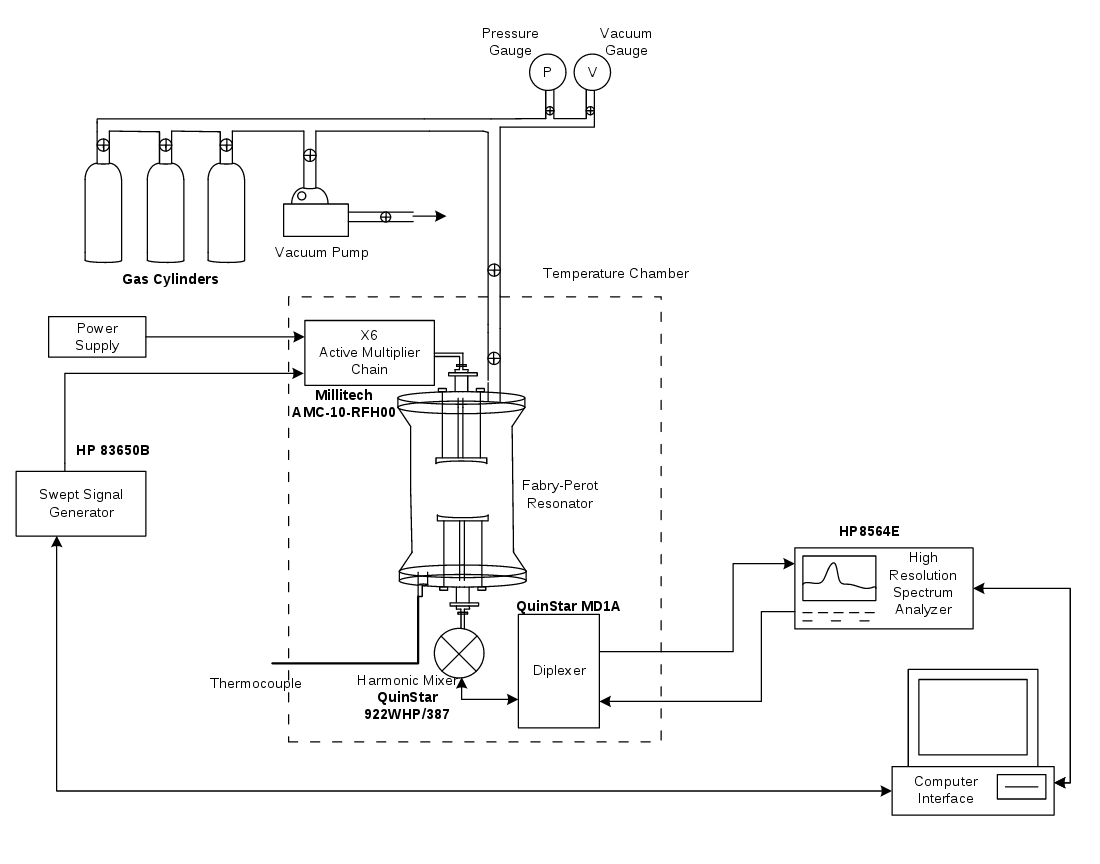
\includegraphics[width=1\textwidth]{./images/w-bandsystem.png}
	\caption{Block diagram of the W-band measurement system. Solid lines represent the electrical connections and the arrows show the direction of the signal propagation. Valves controlling the flow of gasses are shown by small crossed circles.}
    \label{fig:wbandimage}
\end{figure}


\subsection{F-band Subsystem}
The F-band measurement system is used to measure the 2-3 mm-wavelength properties of sulfur dioxide and is shown in figure \ref{fig:fbandimage}.

The swept signal generator (HP 83650B) is used to generate a signal in the 33-50 GHz range which
is amplified and fed through a frequency tripler. The output of the tripler is fed to the input of the FPR via WR-8 waveguides. The RF signal from the output port of the FPR is fed to a harmonic mixer which can operate with an LO frequency as high as 18 GHz. An external diplexer is used to combine the IF and LO signals. For a particular RF and IF frequency,  the LO frequency can be computed using

\begin{equation} \label{eq:fbandlo}
f_{LO} = \frac{f_{RF} - f_{IF}}{N_H	}
\end{equation}

\noindent where N$_H$ is the lowest integer such that $f_{lo} < 18$ GHzs.

\begin{figure}[H]
    \centering
	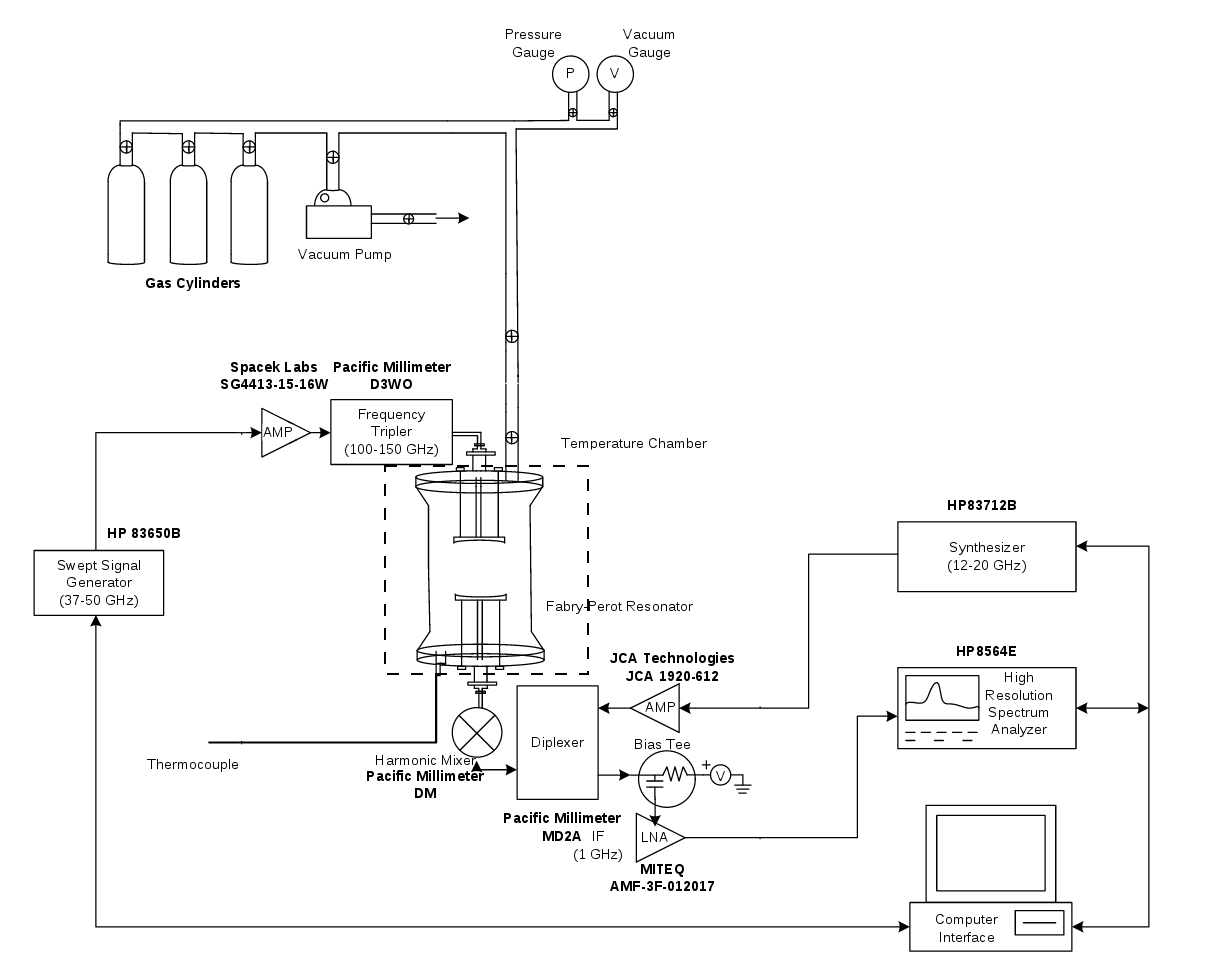
\includegraphics[width=1\textwidth]{./images/f-bandsystem.png}
	\caption{Block diagram of the F-band measurement system. Solid lines represent the electrical connections and the arrows show the direction of the signal propagation. Valves controlling the flow of gasses are shown by small crossed circles.  }
    \label{fig:fbandimage}
\end{figure}

\section{Data Handling Subsystem}

The data acquisition system consists of a computer connected to the spectrum analyzer (HP 8564E), swept signal generator (HP 83650B), and continuous wave (CW) signal generator (HP 83712B, the local oscillator for the F-Band system) via a general purpose interface bus (GPIB). The instruments are controlled via Matlab script and their appropriate programming language. The software used is similar to Devaraj and Steffes \cite{Devaraj-thesis, Devaraj-2011} with modifications for equipment changes.

\section{Measurement Procedure}

The most important prerequisite for performing measurement of gas properties is ensuring a leak-proof system. This is done through two methods, the first method is by drawing a vacuum inside the FPR and verifying the integrity of the vacuum over time. The second method is by adding a positive pressure of CO$_2$ to the system and making sure there are no leaks in any of the connectors and valves. Ensuring a leak-proof system allows for not only precise measurements but also ensures no toxic gases are released into the testing environment.

After the system is ensured to be leak-proof and at a stable temperature, a vacuum is drawn and a measurement is taken using the appropriate subsystem (W-band for 2.7-4.0 mm-wavelengths, F-band for 2-3 mm-wavelengths). This allows for a baseline measurement of the FPR's resonances and the Quality factor. Once this baseline is established the gas under test is added to the system.

Once the gas temperature has stabilized, another set of tests measuring the resonant frequencies along with the quality factors is taken. More gas is added and the procedure is repeated until measurements at all suitable pressures are taken. A vacuum is drawn once again but this time it is pumped overnight due to the possibility of adsorption (or ``sticking'') of the gas being tested (SO$_2$) to metal surfaces inside the vessel. This second vacuum measurement is taken to measure any possible system drift.

Once the second vacuum measurement is taken, CO$_2$ is then added to the chamber until the resonances are matched to the same frequency of our test gas (note that at the pressures and frequencies used for our experiment, pure CO$_2$ is essentially lossless). Again measurements are taken and this is repeated for every pressure of the test gas. Once completed a vacuum is again drawn and another test is taken. 

Lastly the system is set up for a transmissivity test where we measure t (equation \ref{eq:t}) for each given resonant frequency. This is done by by passing the Fabry-Perot resonator and connecting the input and output waveguides through a WR-10 20 dB directional coupler. The signal level is then measured and used to calculate t.  The system is then set back up and is ready for a new test. %Reference table \ref{tab:testmatrix} for the testing matrix being used.


\section{Preliminary Results}

Currently the millimeter-wavelength system is completely operational in the Planetary Atmospheres Laboratory at The Georgia Institute of Technology. Using this system, high precision measurements of SO$_2$'s millimeter-wavelength absorption have recently been completed as part of this work. A preliminary model of SO$_2$'s absorption properties is available from Suleiman's previous work on microwave laboratory measurements \cite{Suleiman-thesis}. Additionally measurements  of SO$_2$'s centimeter-wavelength absorption have recently been taken under deep Venus conditions \cite{so2-cent-lab} \cite{so2-cent-model}. 

\subsection{Millimeter-Wavelength Results}

Only one previous measurement of SO$_2$'s mm-wavelength opacity under Venus simulated conditions has been done (see Fahd et. al. 1991) \cite{fahd-so2} This measurement was done using only one frequency (94.1 GHz) in the mm-wavelength spectra.

In our experiment, eight different frequencies have been already tested using the millimeter-wavelength system measuring 100 mbar of SO$_2$ along with separate tests at 1 bar CO$_2$ combined with the SO$_2$  and 2 bar of CO$_2$ combined with the SO$_2$. This allows for a comparison with Fahd's model and with Suleiman's model at higher frequencies.  

\subsubsection{Absorption Model}

The goal of the laboratory measurements is to create a mathematical model that accurately estimates the opacity of sulfur dioxide in a carbon dioxide atmosphere under all possible conditions of temperature, pressure, concentration, and frequency (fTPC space). For the data fitting process we will use data taken with the FPR along with data from the Planetary Atmospheres Laboratory centimeter-wavelength system  \cite{so2-cent-lab} \cite{so2-cent-model} to create a model that best fits the fTPC space. 

Extrapolating models for SO$_2$'s absorption into the mm-wavelength allows for a good starting point in the model creation process. As visible in the following figures, the absorption model matches the same shape as previous models but is lower by about 20\%. Finding a unified model for SO$_2$'s absorption will compensate for this change.

Figures \ref{fig:so2-116}, \ref{fig:so2-943}, and \ref{fig:so2-1987} show the initial data taken for SO$_2$ opacity in the 3-4 mm-wavelength range. It is clear that previous absorption models work well in predicting the shape of the millimeter-wavelength absorption spectrum of SO$_2$.

\begin{figure}[H]
    \centering
	\includegraphics[width=0.8\textwidth]{./plots/35C_W_High/{0.116-modelComparison}.eps}
	\caption{Measured absorption spectrum given 116 mbar of SO$_2$ at 308K in the W-band range. Shown for comparison are models from Devaraj (2011), Suleiman et al (1996), and Fahd and Steffes (1992).}
    \label{fig:so2-116}
\end{figure}

\begin{figure}[H]
    \centering
	\includegraphics[width=0.8\textwidth]{./plots/35C_W_High/{0.943-modelComparison}.eps}
	\caption{Measured absorption spectrum given 116 mbar of SO$_2$ and 827 mbar of CO$_2$ at 308K in the W-band range.
	Shown for comparison are models from Devaraj (2011), Suleiman et al (1996), and Fahd and Steffes (1992).}
    \label{fig:so2-943}
\end{figure}

\begin{figure}[H]
    \centering
	\includegraphics[width=0.8\textwidth]{./plots/35C_W_High/{1.987-modelComparison}.eps}
	\caption{Measured absorption spectrum given 116 mbar of SO$_2$ and 1871 mbar of CO$_2$ at 308K in the W-band range.
	Shown for comparison are models from Devaraj (2011), Suleiman et al (1996), and Fahd and Steffes (1992).}
    \label{fig:so2-1987}
\end{figure}
\section{Proposed Research}
The objective of the proposed research is to advance the knowledge of the millimeter-wavelength properties of gaseous sulfur dioxide under Venus conditions. As part of the proposed research, extensive laboratory measurements of the W-band and F-band properties of sulfur dioxide under simulated upper Venus atmosphere are ongoing. 

Upon completion of the laboratory measurements, efforts toward developing a unified model to estimate the centimeter and millimeter-wavelength opacity spectra of sulfur dioxide at various pressures, temperatures, and mixing ratios will be developed. 

\subsection{Significance of this Work}
The primary objective of this millimeter-wavelength research is to better understand properties of gaseous sulfur dioxide under Venus conditions. The laboratory measurements will help create a model that accurately estimates the opacity of sulfur dioxide in a carbon dioxide atmosphere at any temperature or pressure. The new model will provide a unified opacity model for sulfur dioxide at the centimeter and millimeter-wavelengths. This model can be used for accurate retrievals of sulfur dioxide from ground-based and spacecraft-based radio observations. 
\subsection{Planned Work}

Two major activities support this thesis: (1) laboratory measurements of 2-4 millimeter-wavelength properties of sulfur dioxide in a carbon dioxide atmosphere at two temperatures, 308 K and 348 K with pressures up to two bars and (2) the development of a model that best estimates sulfur dioxide's millimeter-wavelength absorption properties in Venus's upper troposphere. Both will be completed by Fall Semester 2014.


\subsubsection{Laboratory Measurements}

The ongoing millimeter-wavelength measurements  focus on characterizing the opacity of sulfur dioxide in a carbon dioxide atmosphere temperatures of 308 K and 348 K. These will be the first precision measurements done of sulfur dioxide's absorption properties at millimeter-wavelengths. Previous work by Fahd \cite{fahd-so2} included a measurement done at 94.1 GHz but it did not utilize the high precision measurement tools available for this thesis.  

The testing protocol involve laboratory measurements of the opacity of only sulfur dioxide as well as a mixture of sulfur dioxide and carbon dioxide at pressures of 1 bar and 2 bar. Table \ref{tab:testmatrix} shows a testing matrix of the tests to be done. Varying the sulfur dioxide abundance as well as the temperature allows for an accurate model to be created and extrapolated to other pressure and temperature combinations. 

\begin{table}[H]
    \centering
	\begin{tabular}{|c|c|c|c|c|}
	\hline
	Test Number & Gas under test & Pressure & Temperature & Subsystem\\
	\hline
	\hline
	1 & SO$_2$ & 100 mbar & 308 K & W-band\\
	2 & SO$_2$ & 100 mbar & 343 K & W-band\\
	3 & SO$_2$ & 60 mbar & 343 K & W-band\\
	4 & SO$_2$ & 100 mbar & 343 K & F-band\\
	5 & SO$_2$ & 30 mbar & 343 K & F-band\\
	6 & SO$_2$ & 30 mbar & 308 K & F-band\\
	\hline
	\end{tabular}
	\caption{Testing matrix for SO$_2$'s microwave absorption properties at 2-4 millimeter-wavelength.}
    \label{tab:testmatrix}
\end{table}


\subsubsection{Model Development}

Completed and planned centimeter- \cite{so2-cent-lab} \cite{so2-cent-model} and millimeter-wavelength measurements of the opacity of sulfur dioxide under Venus atmospheric conditions will be used to create a new model that accurately characterizes the centimeter- and millimeter-wavelength properties of sulfur dioxide. After the completion of the millimeter-wavelength laboratory measurements, both centimeter- and millimeter-wavelength data will be put into an optimization algorithm to create the best model estimate of the absorptivity of sulfur dioxide under Venus conditions. 

\subsection{Facilities Required}
All of the facilities required for this work currently exist in the Planetary Atmospheres Laboratory at The Georgia Institute of Technology. The facilities include millimeter-wavelength test equipment, a Fabry-Perot resonator, a temperature chamber, pressure and temperature gauges, and a computer running Matlab. Additional resources that are required and available are gas cylinders of carbon dioxide and sulfur dioxide. Computing resources necessary for model development are available at the Planetary Atmospheres Laboratory.

\subsection{Milestone}

\subsubsection*{Completed Work}
\begin{itemize}
\item Completed setup of millimeter-wavelength system: January 2014
\item Completed 3-4 millimeter-wavelength opacity of SO$_2$ under simulated Venus conditions: February 2014
\item Completed 2-3 millimeter-wavelength opacity of SO$_2$ under simulated Venus conditions: April 2014
\item Diagnosed issue with SO$_2$ pressure regulator and modified data accordingly: April 2014
\item Submit thesis proposal: April 2014
\end{itemize}
\enlargethispage{\baselineskip}
\subsubsection*{Remaining Work}
\begin{itemize}
\item Verify constituent inventory in SO$_2$ bottle and modify data accordingly: April 2014
\item Develop consistent model for opacity of SO$_2$ incorporating the millimeter-wavelength measurements developed as part of this work and the centimeter-wavelength measurements made previously: June 2014
\item Submit journal paper detailing the millimeter-wavelength measurements and the opacity model: November 2014
\item Submit Master's Thesis: December 2014
\end{itemize}

\newpage

\bibliographystyle{elsart-num-sort} 
\bibliography{refs}
\end{document}
